\documentclass[10pt,a4paper]{article}
\usepackage[margin=2.0cm]{geometry}
\usepackage{amsmath,amssymb,booktabs,graphicx,caption,xcolor,microtype,array,float}
\usepackage[hidelinks]{hyperref}
\captionsetup{font=small,labelfont=bf}
\setlength{\parskip}{3pt}
\sloppy
\graphicspath{{figures/}}
\newcommand{\code}[1]{\texttt{\small #1}}
\title{\vspace{-1.2cm}NESS Toy Vertical Slice: Engineering Validation Report}
\author{NESS research platform (generated from run \code{20260926-220302-final})}
\date{2026-09-26}
\begin{document}
\maketitle
\vspace{-0.8cm}
\begin{abstract}
\noindent This report documents the reference run of the NESS synthetic time-series vertical slice: a deterministic two-regime forecasting problem, the instantiated macro-architecture (frozen transformer substrate, trainable upper module, semantic adapter, typed symbolic programs, exact probabilistic regime reasoner, pinned analogue memory, baseline-preserving cap), six matched experiment arms over three model seeds, ten configuration-only substitution proofs, in-run checkpoint/restore identity checks, causal checks, and cost accounting. It is an \emph{engineering validation of interfaces and controls}, not evidence that a neuro-symbolic or probabilistic system beats a Transformer. All numbers and figures are regenerated from saved artifacts by \code{ness report}.
\end{abstract}

\section{Purpose, status and headline findings}
The slice exercises the complete prediction $\rightarrow$ record $\rightarrow$ outcome $\rightarrow$ learning path, port-level substitution of every macro layer, typed symbolic and probabilistic evidence entering one evidence graph, optional causally isolated memory, baseline parity at neutral initialisation, and whole-system checkpoint identity. Status of this run: 18 arm/seed combinations ran to completion (0 failed); 12/12 substitution variants passed every applicable check without any change to core scheduler/runtime source (identical core source hash \code{cbf471e80120}); checkpoint restore reproduced predictions with maximum absolute difference 0.0e+00; every arm passed the target-free causal check. Predictive differences between arms are small on this toy problem and are reported without any superiority claim (Section~\ref{sec:forecast}).

\section{Toy dataset}
\label{sec:data}
All variables are generated deterministically from seed 2026 (\code{toy\_regime\_dataset}), $T=720$ steps. With $\varepsilon^{x}_t,\varepsilon_t\sim\mathcal N(0,1)$ i.i.d.:
\begin{align}
x_t &= \phi_x\,x_{t-1} + \sigma_x\,\varepsilon^{x}_t, &\phi_x&=0.8,\ \sigma_x=0.3,\\
e_t &= \mathbf 1\{t \bmod P < L\}, &P&=25,\ L=3 \quad\text{(scheduled, known in advance)},\\
r_t &= \lfloor t/S \rfloor \bmod 2 \in\{\textsc{normal}=0,\textsc{shift}=1\}, &S&=90 \quad\text{(hidden; change points recorded)},\\
y_t &= a\,y_{t-1} + b_{r_t}\,x_{t-\ell_{r_t}} + c_{r_t}\,e_t + \sigma_{r_t}\,\varepsilon_t, &a&=0.6,
\end{align}
with $(b_0,\ell_0,c_0,\sigma_0)=(0.4,1,0.5,0.1)$ in \textsc{normal} and $(b_1,\ell_1,c_1,\sigma_1)=(-0.4,2,1.5,0.2)$ in \textsc{shift}: the auxiliary channel enters with a different lag and opposite sign, the event effect triples and the noise doubles. Change points: 90, 180, 270, 360, 450, 540, 630.

\paragraph{Task and access policy.} At each rolling origin $o$ the predictor forecasts $y_{o+1},\dots,y_{o+H}$, $H=4$, from the permitted view: \code{series\_history} $=(y_{o-32:o-1},x_{o-32:o-1})$ and \code{event\_history} (role \emph{observed}) plus \code{event\_future} $=e_{o:o+H-1}$ (role \emph{known\_future}). \code{target\_future} (\emph{outcome\_only}) and \code{true\_regime} (\emph{evaluation\_oracle}) travel in the raw bundle for orchestration and evaluation and are removed by every task view before any node runs; the compiler also refuses to wire them. Splits are chronological over origins (train 411, dev 99, test 169 origins) with a gap of $H$ so no training outcome overlaps a test window. Figure~\ref{fig:data} shows a segment.

\begin{figure}[H]\centering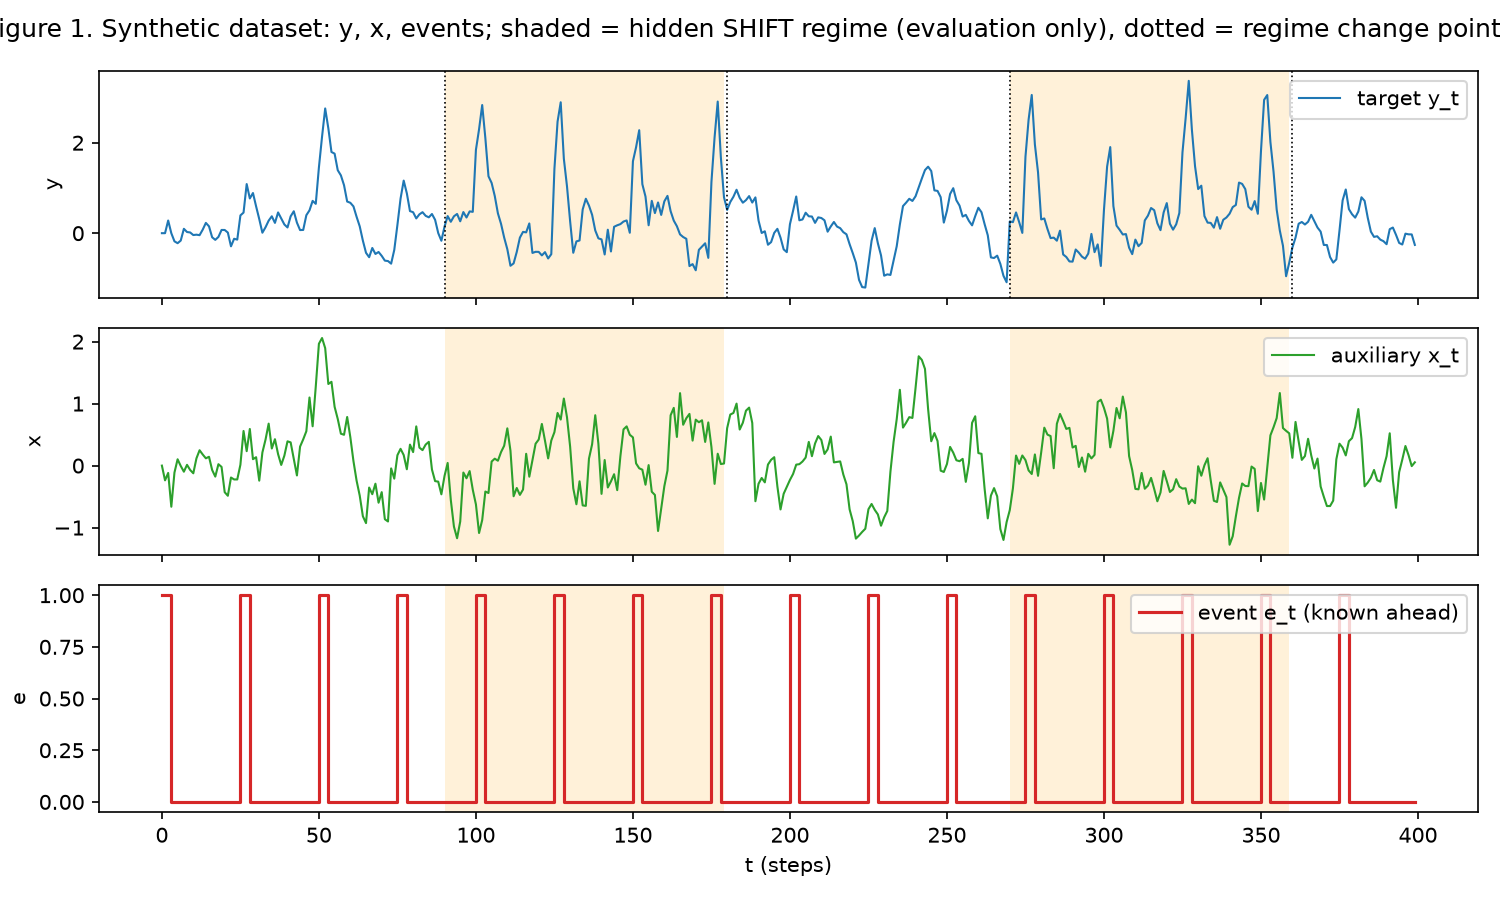
\includegraphics[width=0.92\textwidth]{fig01_dataset.png}
\caption{Synthetic dataset: target $y_t$, auxiliary $x_t$ and scheduled events $e_t$; shaded regions mark the hidden \textsc{shift} regime (evaluation only), dotted lines the regime change points.}\label{fig:data}\end{figure}

\section{Instantiated architecture}
\label{sec:arch}
Figure~\ref{fig:arch} is drawn from the resolved manifest of the full arm (A4), not from the conceptual diagram. Nodes and their roles:
\begin{itemize}\setlength{\itemsep}{1pt}
\item \textbf{Frozen substrate} \code{toy\_frozen\_transformer} (numpy): a genuinely executed 2-block, width-16, 2-head causal transformer encoder with sinusoidal positions and per-window standardisation. It exposes \code{state/early} (after block 1), \code{state/final} and a native point forecast from a ridge-fitted readout ``pretrained'' on an independent synthetic process (its own seed, never the scenario). Group \code{frozen}; explicit stop-gradient boundary.
\item \textbf{Upper module} \code{tiny\_upper\_transformer} (jax): one pre-LN causal block, model width 16. Its input is \code{gated\_add}(\code{state/final}, \code{linear}(\code{state/early})) followed by \code{layer\_norm}; the projection, gate and norm parameters are edge parameters (\code{composition:boundaries}), trainable.
\item \textbf{Semantic adapter} \code{simple\_temporal\_semantics}: reads the raw series directly, the upper hidden state and the known-future events; emits eight typed \code{FeatureEvidence} values: slopes and volatilities of $y$ and $x$ over the last 8 steps, cross-lag correlations $\hat\rho(y_t,x_{t-1})$, $\hat\rho(y_t,x_{t-2})$, a neural cue and an event cue, each with knownness and provenance naming the ports actually consumed.
\item \textbf{Typed programs} (reference interpreter, fuel-bounded): \code{window\_slope\_8} on the series and \code{event\_active\_at\_origin\_h4}, a bounded predicate on the known-future window, $\mathbf 1\{\exists\,h<H:\ e_{o+h}=1\}$. Unknown outputs stay unknown (never silently 0).
\item \textbf{Exact regime reasoner} \code{exact\_finite\_regime\_reasoner}: two latent states, diagonal-Gaussian emissions over the eight semantic features, exact enumeration
\begin{equation}
p(r\mid \mathbf f)=\frac{\pi_r\prod_{j\in\mathcal K}\mathcal N(f_j;\mu_{r j},s_{r j}^2)}{\sum_{r'}\pi_{r'}\prod_{j\in\mathcal K}\mathcal N(f_j;\mu_{r' j},s_{r' j}^2)},\qquad \mathcal K=\{j: f_j\ \text{known}\},
\end{equation}
emitting \code{HypothesisEvidence} with semantics \code{exact\_posterior}. $\mu,s$ were fitted on the \emph{training split} with the hidden regime used as a fitting label (a declared fit-only asset recorded in the config); the neural cue is given an uninformative scale.
\item \textbf{Memory} \code{in\_memory\_snapshot\_store} + \code{analogue\_memory\_query}: a snapshot of matured episodes (window $+$ continuation, available only once the continuation has matured) is pinned per prediction with cutoff $=$ origin; the query returns the mean continuation of the $k=3$ nearest standardised windows as \code{FeatureEvidence} (all-unknown when nothing is eligible) plus \code{RetrievalEvidence}. The learner appends new matured episodes to a branch and publishes a new snapshot only between updates.
\item \textbf{Cap} \code{residual\_point\_cap}: consumer $=$ zero-initialised linear map from the concatenated evidence (neural, semantic, programs, posterior, memory) to a correction $\Delta\in\mathbb R^{H}$; writer $\hat\mu = \mu_0 + \Delta$. Zero initialisation gives bitwise baseline parity before learning.
\end{itemize}
Learning: profile \code{bp\_direct} (reverse-mode BP through the deployed direct computation) owns the upper, cap and boundary groups; every edge from a host node into the cap is a stop-gradient leaf recorded in the credit map. Inference profile \code{direct}. Task loss and score are the mean squared error over the $H$ horizon steps, reduced as $\sum \text{numerators}/\sum\text{counts}$.

\begin{figure}[H]\centering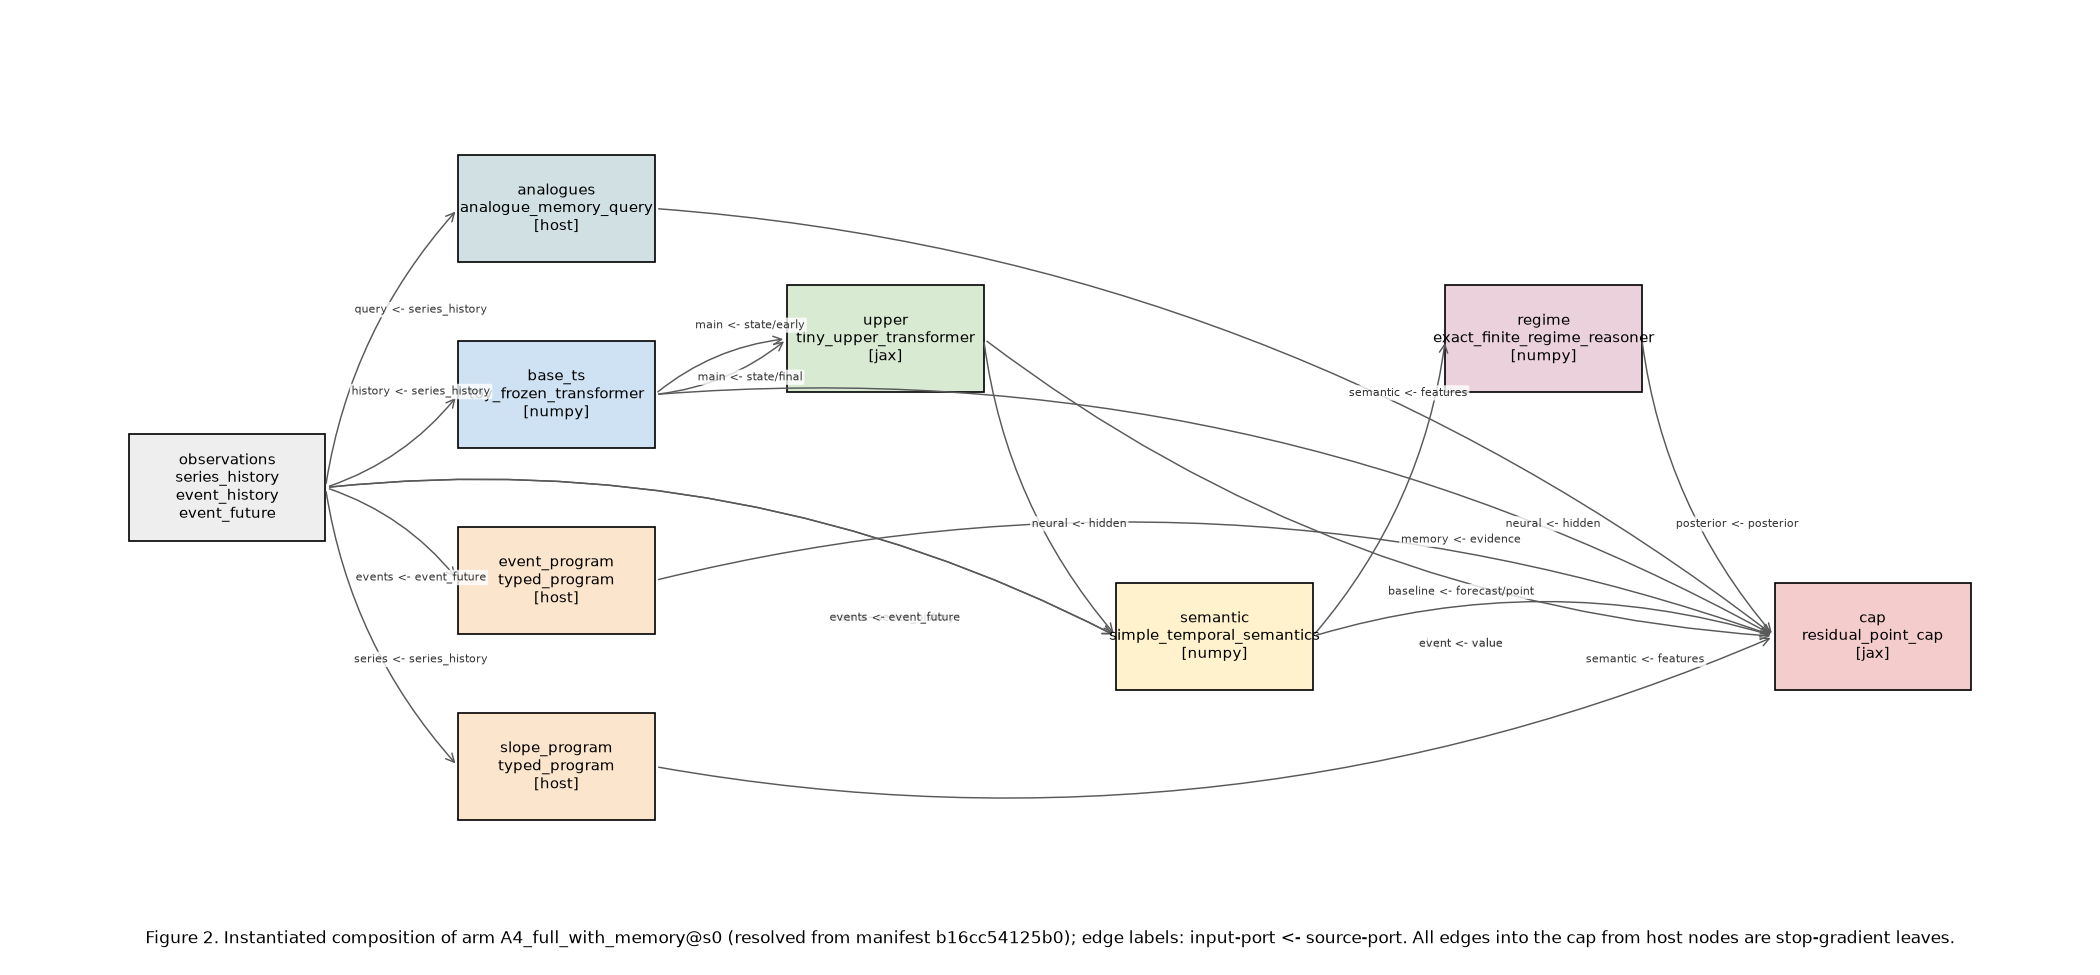
\includegraphics[width=\textwidth]{fig02_architecture.png}
\caption{Instantiated composition of arm A4 generated from its manifest (\code{ness report}). Edge labels read \emph{input-port $\leftarrow$ source-port}; the direct raw-input edge into the semantic layer and the early-state residual into the upper module are visible.}\label{fig:arch}\end{figure}

\section{Experiment arms and protocol}
\begin{center}\small\begin{tabular}{@{}l p{11.8cm}@{}}\toprule
A0 & frozen substrate's native forecast; no learned parameters\\
A1 & A0 $+$ trainable upper transformer (final $+$ projected early residual) $+$ residual cap\\
A2 & A1 $+$ semantic adapter (raw, upper state, events) $+$ typed slope and event programs\\
A3 & A2 $+$ exact two-state regime posterior\\
A4 & A3 $+$ pinned analogue memory\\
A5 & same-fact neural control: the $32\times2$ raw window and the known-future events enter the cap directly (68 dense features); no symbolic computation\\
\bottomrule\end{tabular}\end{center}
Every arm sees identical request streams. Model seeds [0, 1, 2] (dataset seed locked); prequential training with batches of 8 requests and 24 Adam updates (lr $3\cdot10^{-3}$, gradient-norm clip 5), then frozen evaluation on 169 test origins (no parameter, count or memory updates). After training, a whole-system learner checkpoint is published and restored, and the first 16 test requests are re-predicted by the restored system; a causal check re-predicts a request with its withheld outcome fields perturbed and removed. Wall-clock per phase and process peak RSS are recorded.

\section{Forecasting results}
\label{sec:forecast}
\begin{table}[H]\centering\small
\caption{Test error on all horizons, mean $\pm$ sd over 3 model seeds. ``Transition'' = origins within 8 steps of a regime change. Differences are engineering smoke results on one synthetic dataset and support no superiority claim.}
\begin{tabular}{@{}lccccrr@{}}\toprule
arm & MAE & RMSE & MAE stable & MAE transition & scored & failed\\\midrule
A0\_frozen\_baseline & 0.646 $\pm$ 0.000 & 0.853 & 0.676 & 0.391 & 169 & 0\\
A1\_neural\_cap & 0.624 $\pm$ 0.017 & 0.836 & 0.655 & 0.363 & 169 & 0\\
A2\_neural\_symbolic & 0.608 $\pm$ 0.017 & 0.818 & 0.640 & 0.344 & 169 & 0\\
A3\_neural\_symbolic\_probabilistic & 0.607 $\pm$ 0.017 & 0.817 & 0.639 & 0.345 & 169 & 0\\
A4\_full\_with\_memory & 0.594 $\pm$ 0.017 & 0.802 & 0.626 & 0.324 & 169 & 0\\
A5\_same\_fact\_neural & 0.524 $\pm$ 0.007 & 0.717 & 0.556 & 0.260 & 169 & 0\\
\bottomrule\end{tabular}\label{tab:metrics}\end{table}
All learned caps reduce the frozen baseline's test MAE (0.646) by roughly 8\% (Table~\ref{tab:metrics}); the lowest mean MAE is A5\_same\_fact\_neural (0.524). The spread between the trainable arms (0.099) is of the same order as the across-seed standard deviation (typically 0.015), so the ordering among A1--A5 is not resolved by this run. In particular the symbolic and probabilistic arms are not shown to beat the same-fact neural control A5; this is a null result on the toy problem, reported as such. Error rises near regime transitions for every arm (right panel of the next figure), the mechanism the toy was built to expose.
\begin{figure}[H]\centering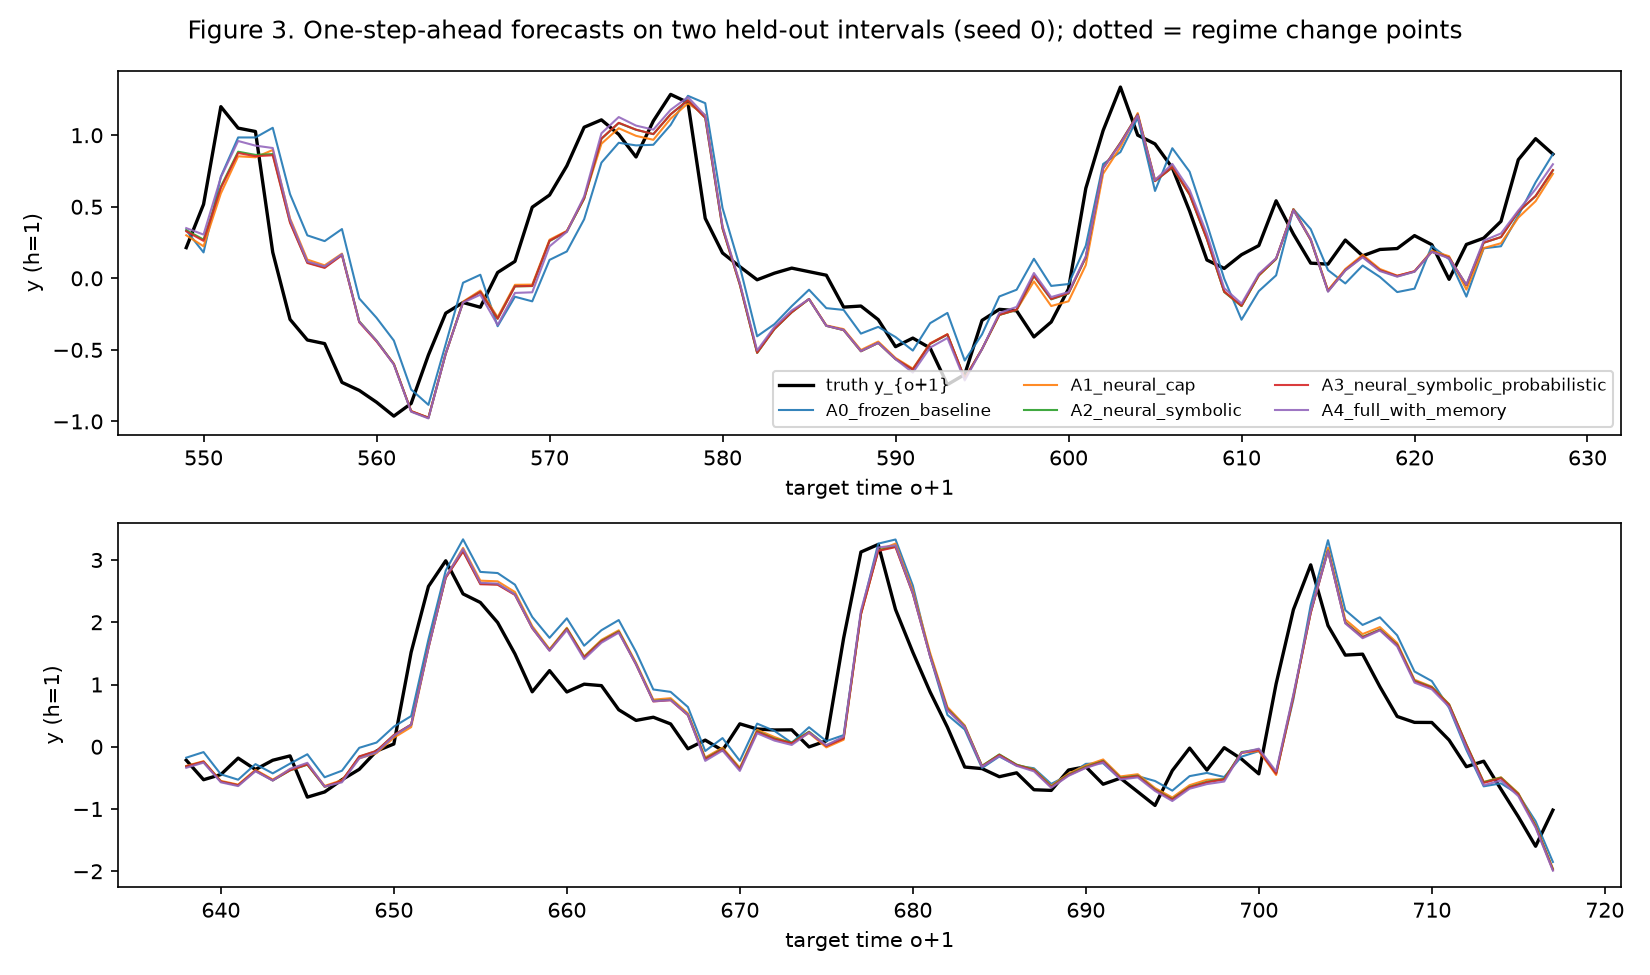
\includegraphics[width=\textwidth]{fig03_trajectories.png}
\caption{One-step-ahead forecasts on two held-out intervals (seed 0) against the truth; dotted lines mark regime changes.}\end{figure}
\begin{figure}[H]\centering
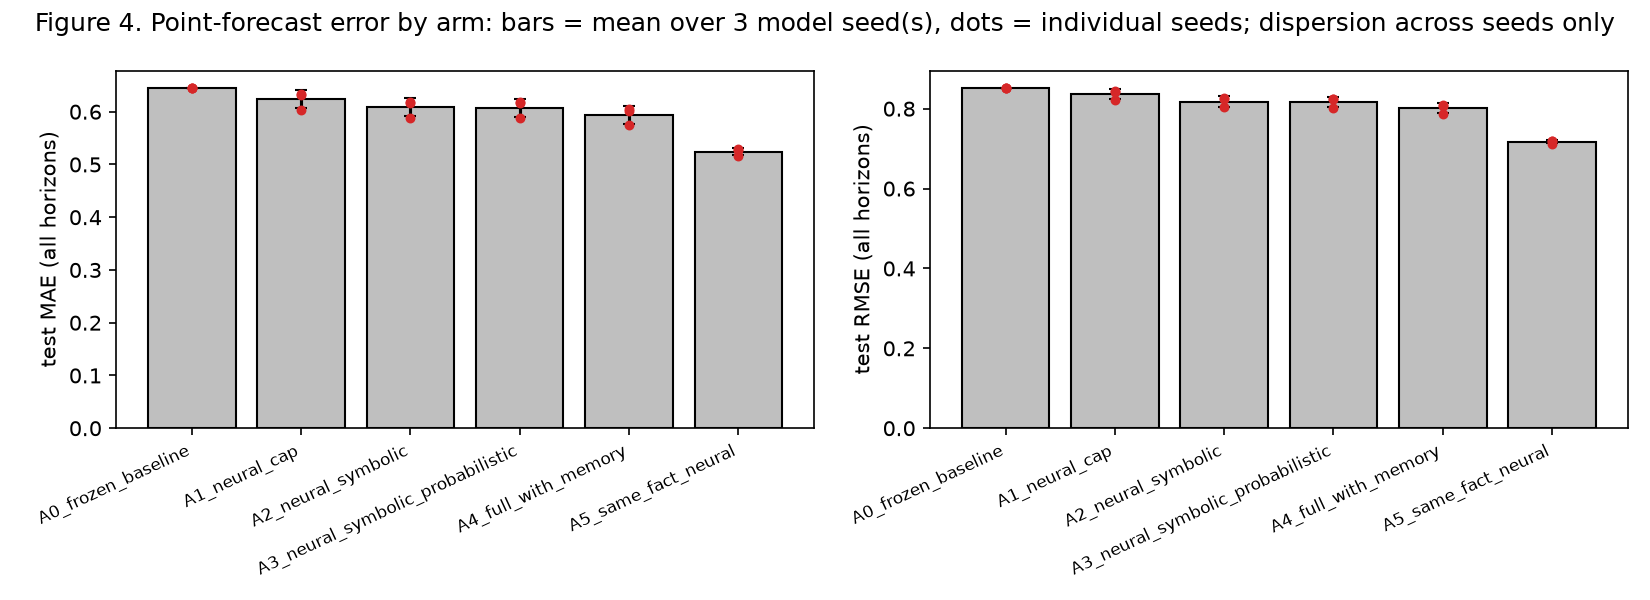
\includegraphics[width=0.58\textwidth]{fig04_metric_by_arm.png}\hfill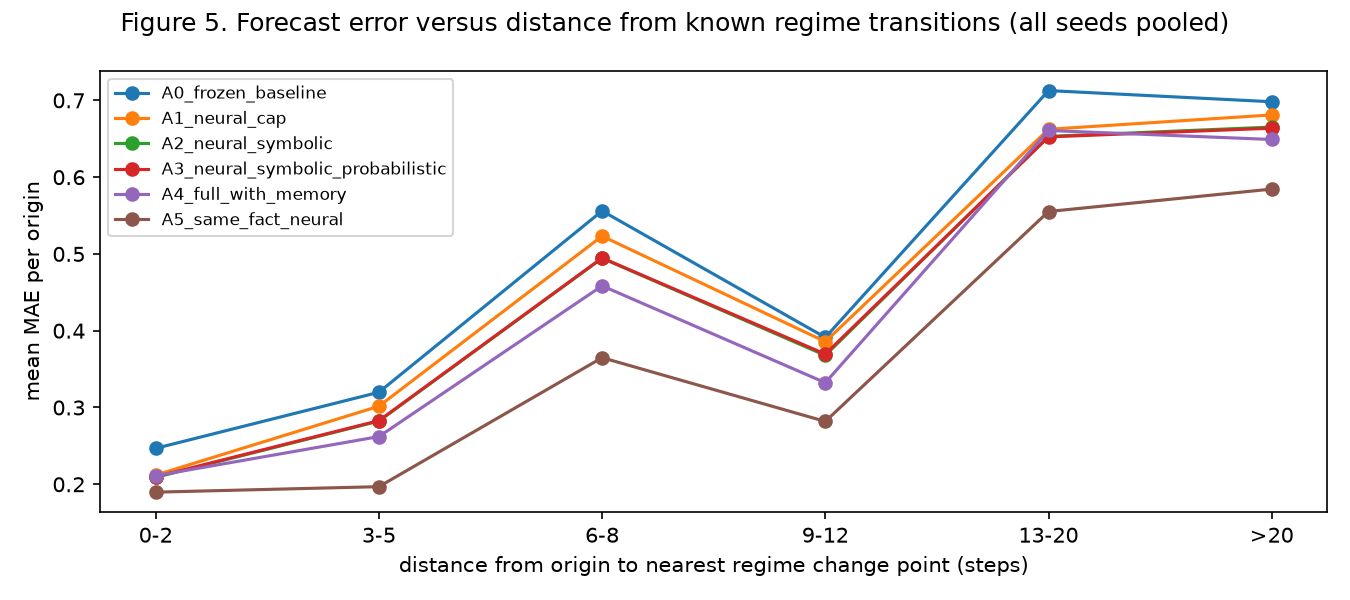
\includegraphics[width=0.41\textwidth]{fig05_error_vs_transition.png}
\caption{Left: MAE/RMSE by arm (bars: mean over seeds; dots: seeds). Right: per-origin MAE versus distance to the nearest regime change point.}\end{figure}

\section{Probabilistic, symbolic and memory diagnostics}
\paragraph{Regime posterior.} Against the hidden regime at the origin (evaluation only), the exact posterior scores A3\_neural\_symbolic\_probabilistic: accuracy 0.811, Brier 0.143, NLL 0.431; A4\_full\_with\_memory: accuracy 0.811, Brier 0.143, NLL 0.431 over 169 test origins per seed (posterior semantics \code{exact\_posterior}, omitted mass 0). Errors concentrate in the first origins after a change point, where the 8-step feature window still straddles both regimes (Figure~\ref{fig:post}). The reasoner never sees the hidden regime; its inputs are the eight permitted semantic features. Figure~\ref{fig:post} overlays $p(\textsc{shift}\mid\mathbf f)$ on the evaluation-only truth.
\begin{figure}[H]\centering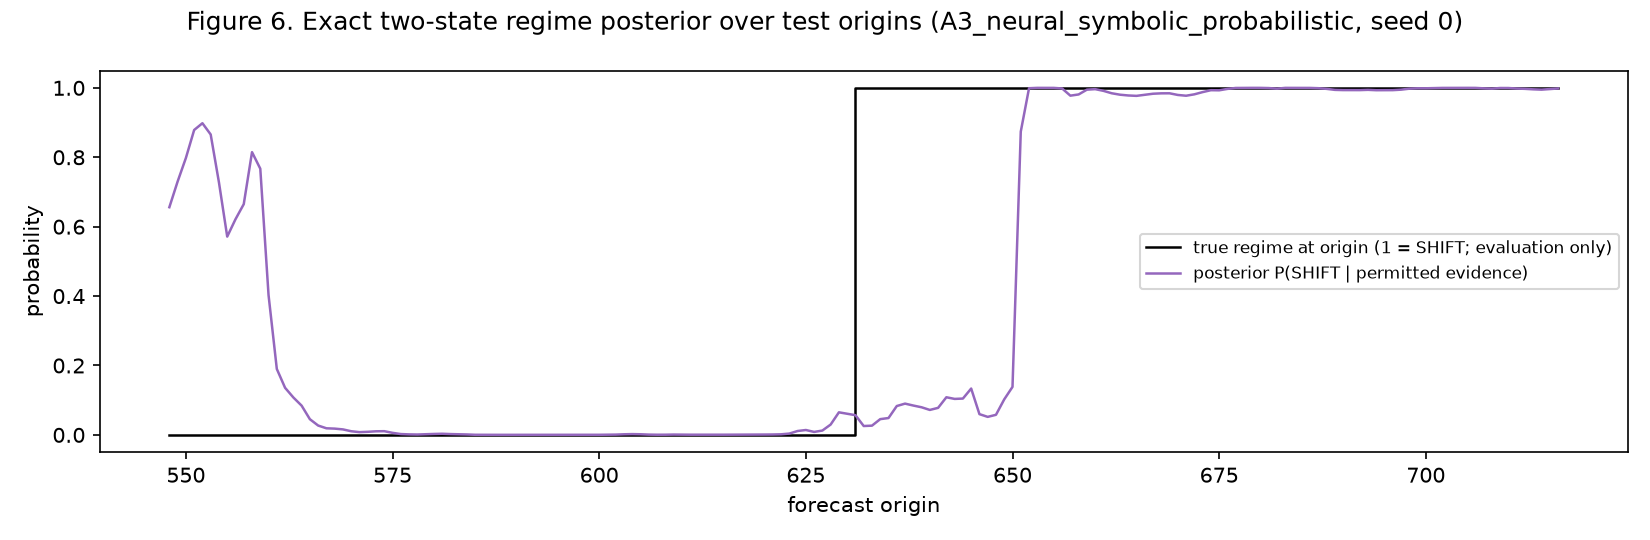
\includegraphics[width=\textwidth]{fig06_regime_posterior.png}
\caption{Exact two-state posterior over test origins (A3, seed 0) versus the hidden regime.}\label{fig:post}\end{figure}
\paragraph{Symbolic pathway.} The typed event predicate agreed with the ground-truth ``event within horizon'' on 100.0\% of 169 test origins with 100\% known outputs (no unknown/error states occurred: the known-future window is always complete). The semantic features separate the regimes as designed: mean $\hat\rho(y_t,x_{t-1})$ = 0.58 (\textsc{normal}) vs -0.52 (\textsc{shift}); volatility of $y$ 0.28 vs 0.44. Mean $|$slope$_y|$: 0.104 vs 0.180. Adding the symbolic path changed the cap's predictions (paired test-loss delta vs A0: A1 -0.028, A2 -0.059, mean over seeds), but the change is within seed dispersion.
\paragraph{Memory.} 1083 retrievals were issued (train and test phases); 1.1\% returned no eligible analogue (early training origins before any episode had matured). Retrieved episodes were on average 230 steps old (median 127, minimum 4 $\geq H$), none truncated. Paired A3$\to$A4 test-loss deltas per seed: [-0.023, -0.025, -0.024], i.e.\ no measurable effect of memory here.
\begin{figure}[H]\centering
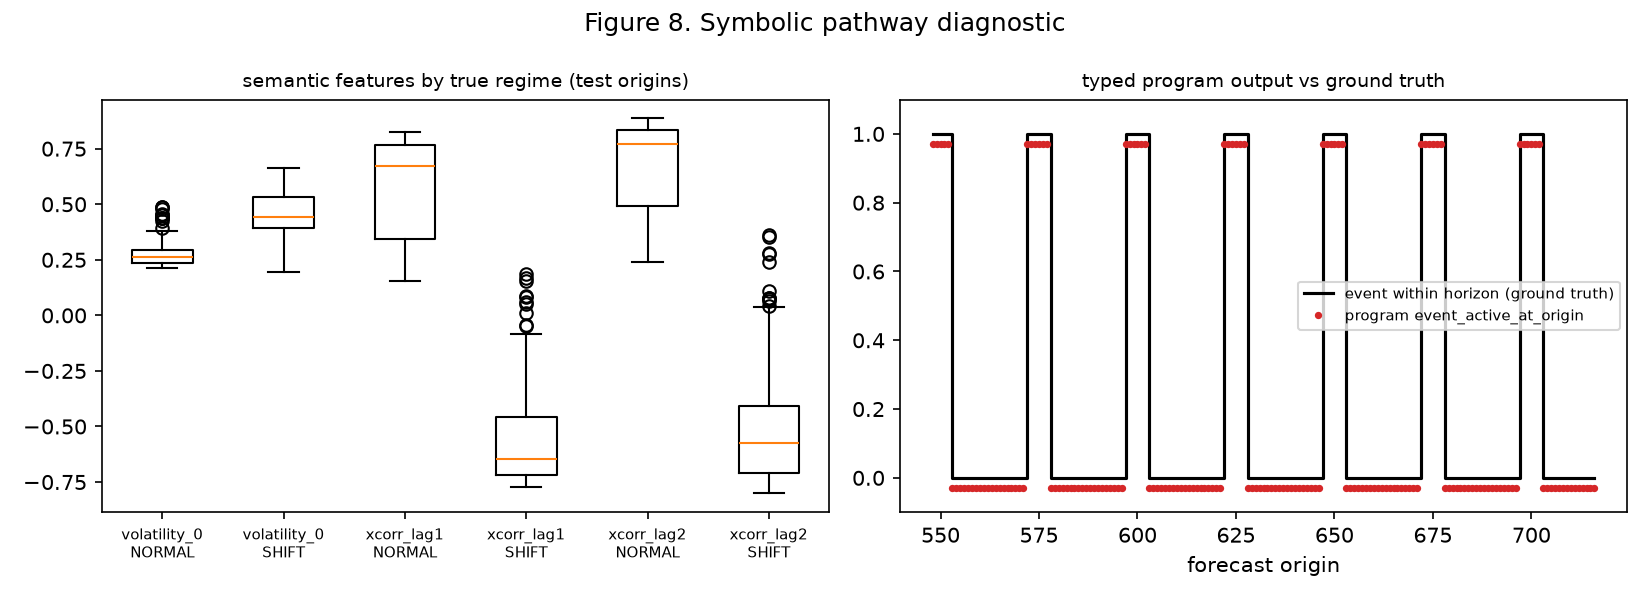
\includegraphics[width=0.56\textwidth]{fig08_symbolic.png}\hfill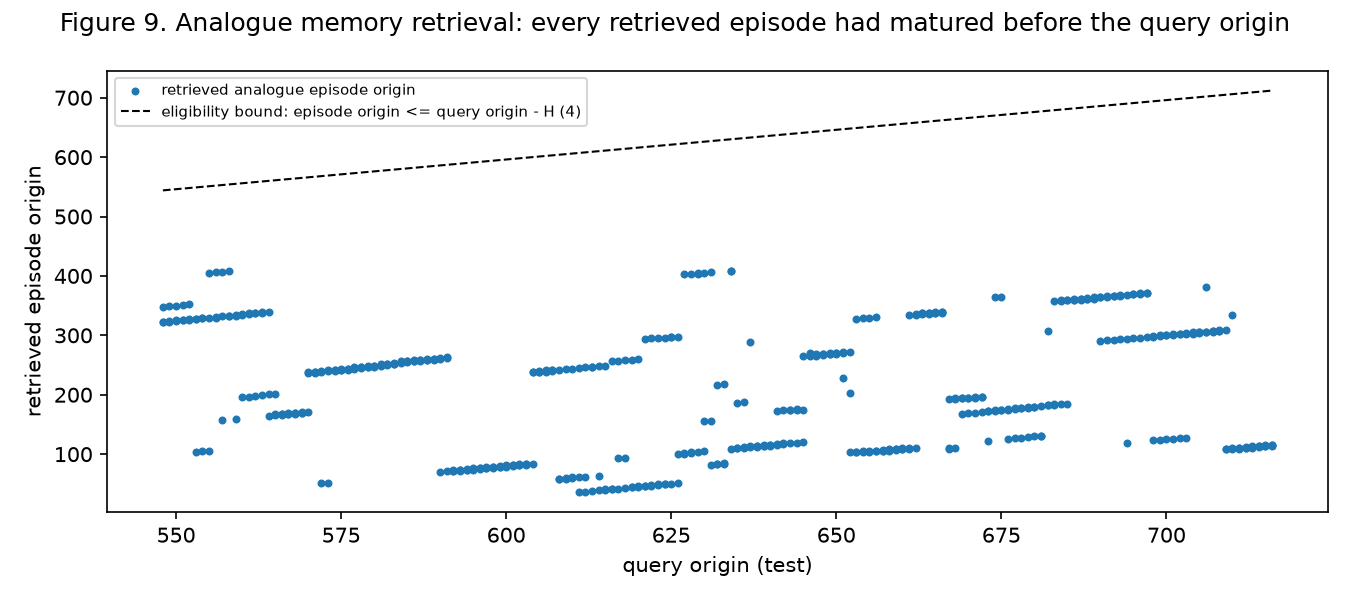
\includegraphics[width=0.43\textwidth]{fig09_memory_retrieval.png}
\caption{Left: semantic features split by true regime and the event predicate against ground truth. Right: retrieved analogue origins versus query origin; all points lie below the eligibility bound (episode matured before the origin).}\end{figure}

\section{Training dynamics and cost}
\begin{figure}[H]\centering
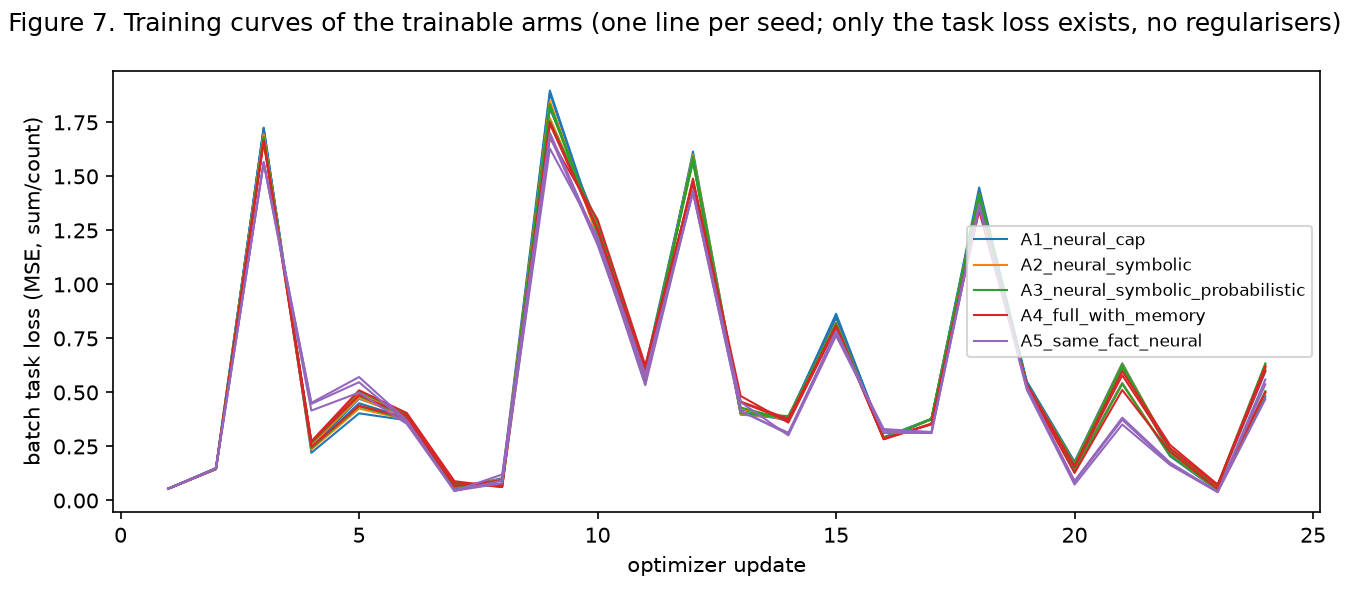
\includegraphics[width=0.5\textwidth]{fig07_training_curves.png}\hfill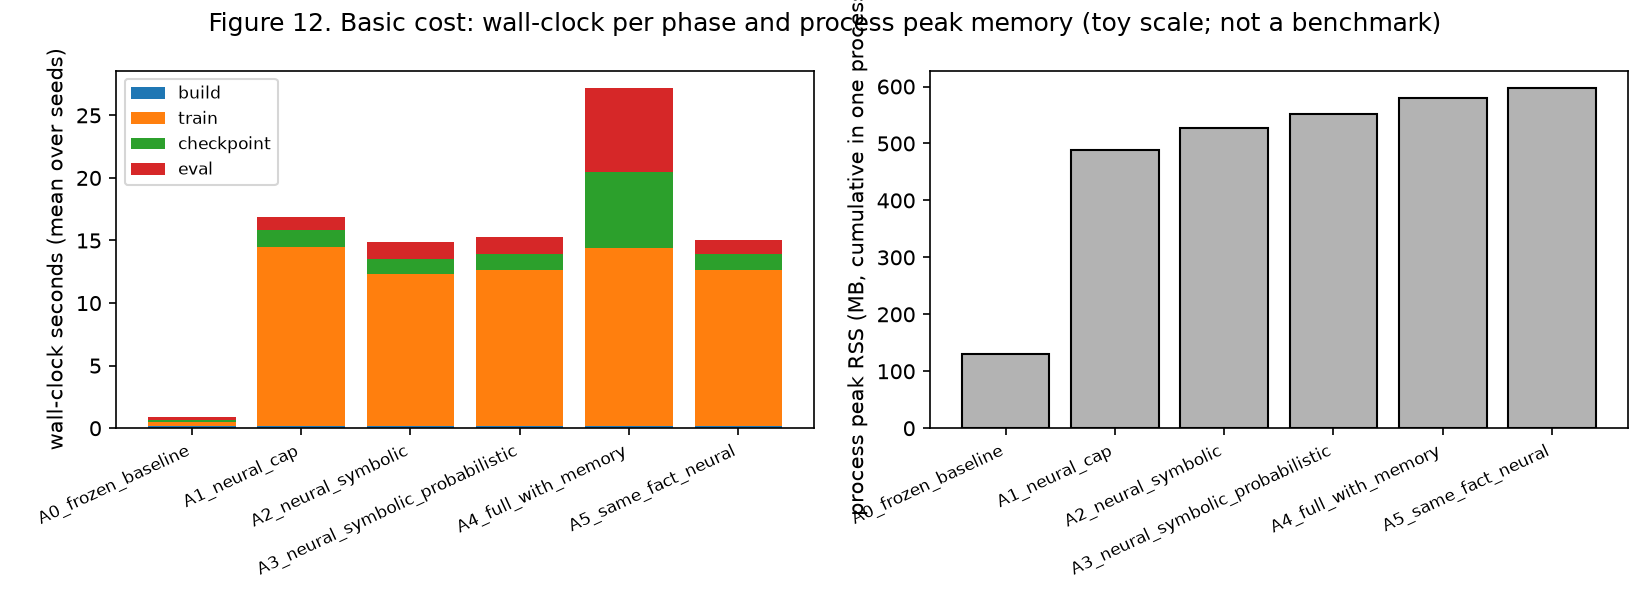
\includegraphics[width=0.49\textwidth]{fig12_cost.png}
\caption{Left: batch task loss per update for the trainable arms (one line per seed). Right: wall-clock per phase and process peak RSS (toy scale, not a benchmark).}\end{figure}
The batch loss falls from 0.055 to 0.565 on average over 24 updates for every trainable arm and seed; no non-finite state, clipping fallback or failed run occurred. Wall-clock per arm is dominated by per-request reverse-mode tracing (\code{metrics/timing.csv}); the semantic/program/reasoner/memory host nodes add visible but small cost.

\section{Modularity, checkpoint identity and acceptance}
\begin{table}[H]\centering\scriptsize
\caption{Substitution matrix: each row is a complete arm built by configuration only; checks are validate/compile, target-free prediction, causal invariance, one training update (where trainable) and checkpoint restore identity. Core source hash identical for all rows.}
\begin{tabular}{@{}l >{\raggedright\arraybackslash}p{5.4cm} ccccc@{}}\toprule
id & description & validate & predict & causal & train & restore\\\midrule
S01\_lower\_provider\_conv & lower provider A (transformer) $\to$ provider B (causal conv) & pass & pass & pass & pass & pass\\
S02\_upper\_mlp & upper transformer $\to$ MLP upper module & pass & pass & pass & pass & pass\\
S03a\_semantic\_raw\_only & semantic adapter reads raw input only & pass & pass & pass & pass & pass\\
S03b\_semantic\_base\_final\_only & semantic adapter reads raw (required) + base final state instead of the upper state & pass & pass & pass & pass & pass\\
S03c\_semantic\_raw\_plus\_final & semantic adapter reads raw + base final & pass & pass & pass & pass & pass\\
S03d\_semantic\_raw\_early\_final & semantic adapter reads raw + early (neural port) + final (base\_context port) & pass & pass & pass & pass & pass\\
S04\_residual\_off & early-state residual into the upper module disabled & pass & pass & pass & pass & pass\\
S05\_rms\_norm & boundary normalisation layer\_norm $\to$ rms\_norm & pass & pass & pass & pass & pass\\
S06\_programs\_disabled & symbolic programs removed (semantic adapter kept) & pass & pass & pass & pass & pass\\
S07\_trivial\_reasoner & exact reasoner $\to$ deterministic threshold reasoner (external plugin) & pass & pass & pass & pass & pass\\
S08\_memory\_disabled & memory removed from the full cap & pass & pass & pass & pass & pass\\
S09\_writer\_consumer\_changed & bounded writer (external plugin) + MLP consumer & pass & pass & pass & pass & pass\\
\bottomrule\end{tabular}\label{tab:subs}\end{table}
\begin{figure}[H]\centering
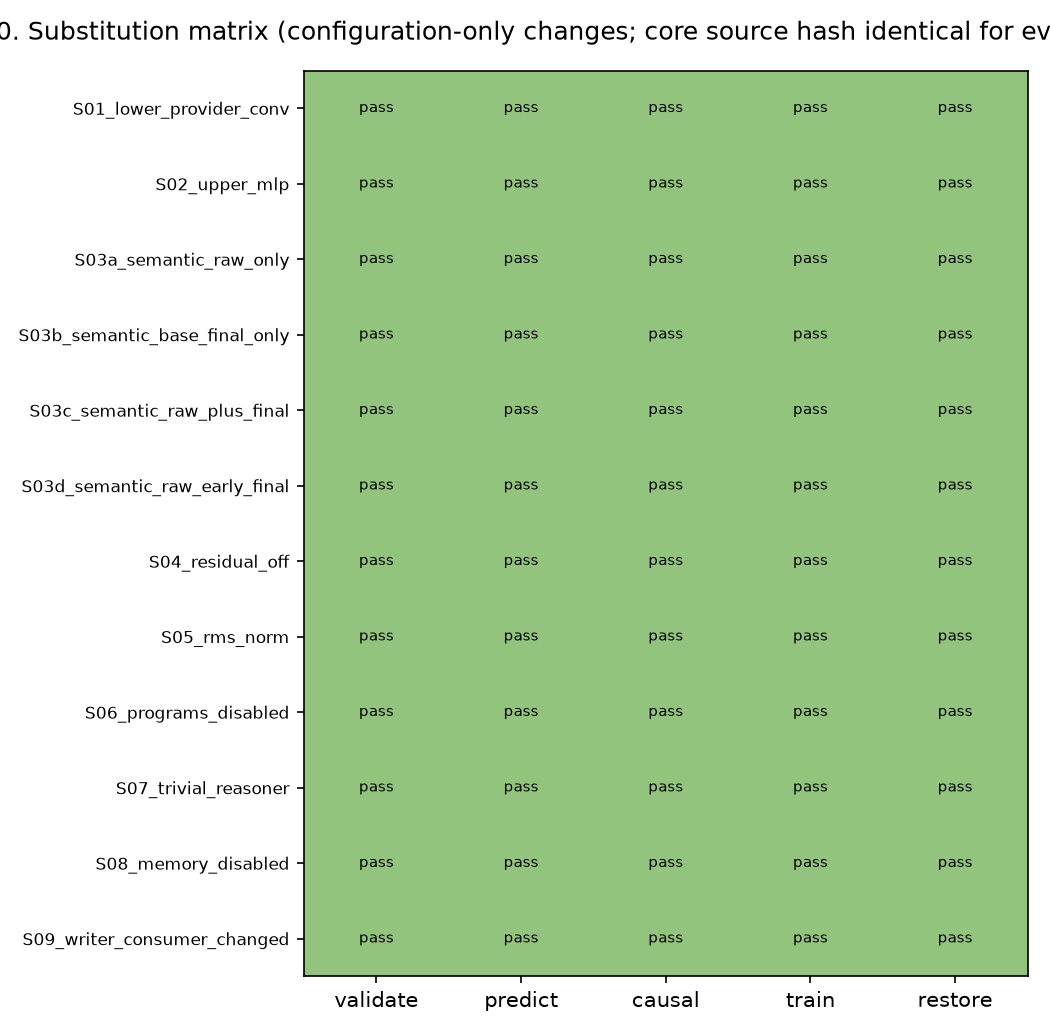
\includegraphics[width=0.52\textwidth]{fig10_substitution_matrix.png}\hfill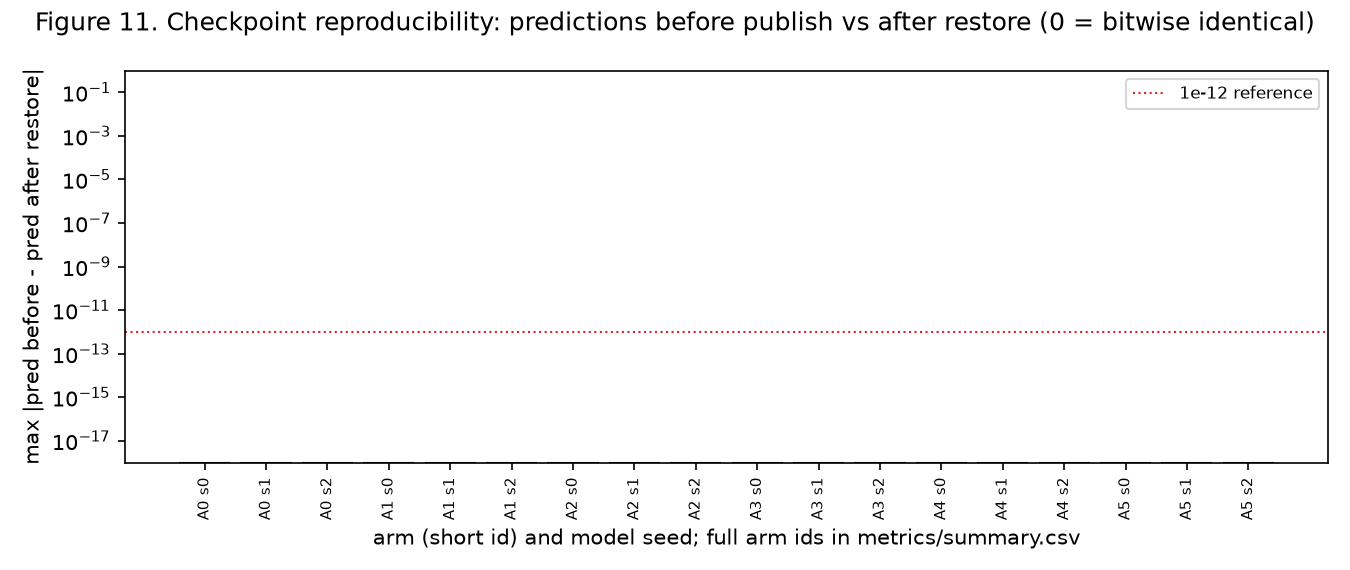
\includegraphics[width=0.47\textwidth]{fig11_checkpoint_restore.png}
\caption{Left: substitution matrix. Right: maximum absolute prediction difference before checkpoint publication and after restore, per arm and seed (bars at the floor are exactly zero).}\end{figure}
Every arm/seed published a learner checkpoint (content-addressed blobs, expected-parent compare-and-swap) and was restored by manifest; the restored predictor reproduced the first 16 test predictions with maximum absolute difference 0.0e+00 and its manifest id matched in every case. Manifest ids are listed in \code{metrics/summary.json} and \code{manifests/}.

\paragraph{Acceptance mapping.} Exercised by this run: T04/T38 (causal invariance per arm and per substitution), T08/T27/T40 (publish with compare-and-swap, restore identity, plugin state round trips), T18 (baseline parity at zero correction), T31/T33--T35 (provider, upper, routing, residual, normalisation substitutions), T36 (compile-time recurrence policy, via the suite), T37 (reasoner substitution S07), T39 (memory isolation in A4), T43 (resolved wiring in manifests), T44 (outcome fields excluded from views). Not applicable at this scale: T10, T12, T14, T20, T25--T29, T32. Full test-suite status: full platform suite at the time of this fill: 204 passed, 3 environment/contract skips, 0 failed of 207 collected (CPU, \texttt{pytest -p no:cacheprovider}, 2\,min); the tiny pipeline test \code{tests/test\_toy\_slice\_pipeline.py} exercises this run's code path.

\section{Problems found, decisions, and next steps}
\begin{itemize}\setlength{\itemsep}{1pt}
\item Fitted emission parameters of the exact reasoner are configuration today; a fitted-state contract would make them first-class plugin state with their fitting population recorded (ADR candidate).
\item The reference cap lowers unknown feature entries to 0 and does not consume knownness masks (declared capability); a mask-aware consumer is a plugin change, not a core change.
\item Per-request tracing under reverse-mode differentiation dominates training time at this scale; batched/data-parallel evaluation exists for uniform shapes.
\item The memory query window had to declare its channel count separately from the continuation channels (\code{query\_channels}); this was a general interface gap fixed in the plugin, not a toy-specific patch.
\item Next integrations, smallest first: a TimesFM-3 forecast-only substrate behind the same \code{forecast/point|quantiles} ports; a frozen text$+$vision substrate pair with alignment evidence; a Hyperon-backed \code{MemoryStore}; a NumPyro reasoner compared against the exact one; larger frozen-provider runs on the FabricPC backend.
\end{itemize}
\paragraph{Reproduction.} \code{ness validate examples/vertical\_slice\_timeseries/configs/toy\_vertical\_slice.yaml}; \code{ness run \ldots\ --out <run>}; \code{ness evaluate <run>}; \code{ness report <run>}; \code{ness inspect <run>/checkpoints <manifest>}. Raw artifacts (CSV/JSON) and the Markdown report live under the run directory; this document was filled from them by \code{reports/fill\_report.py}.
\end{document}
